\documentclass[a4paper,11pt]{article}
\usepackage{amsmath,amsthm,amsfonts,amssymb,amscd,amstext,vmargin,graphics,graphicx,tabularx,multicol} \usepackage[french]{babel}
\usepackage[utf8]{inputenc}  
\usepackage[T1]{fontenc} 
\usepackage[T1]{fontenc}
\usepackage{amsmath,amssymb}
\usepackage{pstricks-add,tikz,tkz-tab,variations}
\usepackage[autolanguage,np]{numprint} 

\setmarginsrb{1.5cm}{0.5cm}{1cm}{0.5cm}{0cm}{0cm}{0cm}{0cm} %Gauche, haut, droite, haut
\newcounter{numexo}
\newcommand{\exo}[1]{\stepcounter{numexo}\noindent{\bf Exercice~\thenumexo} : \marginpar{\hfill /#1}}
\reversemarginpar


\newcounter{enumtabi}
\newcounter{enumtaba}
\newcommand{\q}{\stepcounter{enumtabi} \theenumtabi.  }
\newcommand{\qa}{\stepcounter{enumtaba} (\alph{enumtaba}) }
\newcommand{\initq}{\setcounter{enumtabi}{0}}
\newcommand{\initqa}{\setcounter{enumtaba}{0}}

\newcommand{\be}{\begin{enumerate}}
\newcommand{\ee}{\end{enumerate}}
\newcommand{\bi}{\begin{itemize}}
\newcommand{\ei}{\end{itemize}}
\newcommand{\bp}{\begin{pspicture*}}
\newcommand{\ep}{\end{pspicture*}}
\newcommand{\bt}{\begin{tabular}}
\newcommand{\et}{\end{tabular}}
\renewcommand{\tabularxcolumn}[1]{>{\centering}m{#1}} %(colonne m{} centrée, au lieu de p par défault) 
\newcommand{\tnl}{\tabularnewline}

\newcommand{\trait}{\noindent \rule{\linewidth}{0.2mm}}
\newcommand{\hs}[1]{\hspace{#1}}
\newcommand{\vs}[1]{\vspace{#1}}

\newcommand{\N}{\mathbb{N}}
\newcommand{\Z}{\mathbb{Z}}
\newcommand{\R}{\mathbb{R}}
\newcommand{\C}{\mathbb{C}}
\newcommand{\Dcal}{\mathcal{D}}
\newcommand{\Ccal}{\mathcal{C}}
\newcommand{\mc}{\mathcal}

\newcommand{\vect}[1]{\overrightarrow{#1}}
\newcommand{\ds}{\displaystyle}
\newcommand{\eq}{\quad \Leftrightarrow \quad}
\newcommand{\vecti}{\vec{\imath}}
\newcommand{\vectj}{\vec{\jmath}}
\newcommand{\Oij}{(O;\vec{\imath}, \vec{\jmath})}
\newcommand{\OIJ}{(O;I,J)}

\newcommand{\bmul}[1]{\begin{multicols}{#1}}
\newcommand{\emul}{\end{multicols}}


\newcommand{\reponse}[1][1]{%
\multido{}{#1}{\makebox[\linewidth]{\rule[0pt]{0pt}{20pt}\dotfill}
}}

\newcommand{\titre}[5] 
% #1: titre #2: haut gauche #3: bas gauche #4: haut droite #5: bas droite
{
\noindent #2 \hfill #4 \\
#3 \hfill #5

\vspace{-1.6cm}

\begin{center}\rule{6cm}{0.5mm}\end{center}
\vspace{0.2cm}
\begin{center}{\large{\textbf{#1}}}\end{center}
\begin{center}\rule{6cm}{0.5mm}\end{center}
}



\begin{document}
\pagestyle{empty}
\titre{Correction de l'interrogation sur les fractions}{Nom :}{Prénom :}{Classe}{Date}



\exo{6.5}

\bmul{4}

$R = \dfrac{6}{5} + \dfrac{18}{5} + \dfrac{21}{5}$\\

\red
 $R = \dfrac{6 + 18 +21}{5} $\\

$R = \dfrac{45 \div 5}{5 \div 5} $\\

$R = \dfrac{9}{1} $\\

$\fbox{R =9} $\\
\black

\columnbreak

$E = \dfrac{5}{3} - \dfrac{10}{12}$\\ 

\red

$E = \dfrac{5 \times 4}{3 \times 4} - \dfrac{10}{12}$\\ 

$E = \dfrac{20}{12} - \dfrac{10}{12}$\\ 

$E = \dfrac{20-10}{12}$\\ 

$E = \dfrac{10 \div 2}{12 \div 2}$\\ 

\fbox{$E = \dfrac{5}{6}$}\\ 

\black

\columnbreak

$P = 3 - \dfrac{2}{7}$\\ 

\red

$P = \dfrac{3}{1} - \dfrac{2}{7}$\\ 

$P = \dfrac{3 \times 7}{1 \times 7} - \dfrac{2}{7}$\\ 

$P = \dfrac{21}{7} - \dfrac{2}{7}$\\ 

$P = \dfrac{21 - 2}{ 7} $\\ 

\fbox{$P = \dfrac{19}{ 7} $}\\ 

\black

\columnbreak

$S =\dfrac{1}{3}+\dfrac{4}{5} - \dfrac{11}{45}$\\ 

\red

$S =\dfrac{1 \times 15}{3 \times 15}+\dfrac{4 \times 9}{5 \times 9} - \dfrac{11}{45}$\\ 

$S =\dfrac{15}{45}+\dfrac{36}{45} - \dfrac{11}{45}$\\ 

$S =\dfrac{15 + 36}{45} - \dfrac{11}{45}$\\ 

$S =\dfrac{51}{45} - \dfrac{11}{45}$\\ 

$S = \dfrac{51 - 11}{45}$\\ 

$S = \dfrac{40 \div 5}{45 \div 5}$\\ 

\fbox{$S = \dfrac{8}{9}$}\\ 

\emul

\bmul{2}

$F = \dfrac{21}{4} - \left( \dfrac{1}{2} - \dfrac{1}{4}   \right)$\\ 

\red

$F = \dfrac{21}{4} - \left( \dfrac{1 \times 2}{2 \times 2} - \dfrac{1}{4}   \right)$\\ 

$F = \dfrac{21}{4} - \left( \dfrac{2}{4} - \dfrac{1}{4}   \right)$\\ 

$F = \dfrac{21}{4} - \left( \dfrac{2 - 1}{4}  \right)$\\ 

$F = \dfrac{21}{4} -  \dfrac{1}{4}  $\\ 

$F = \dfrac{21 - 1}{4} $\\ 

$F = \dfrac{20 \div 4}{4 \div 4} $\\ 

$F = \dfrac{5}{1} $\\ 

\fbox{$F = 5 $}\\ 
\black

\columnbreak

$M = \left(  \dfrac{7}{6}+\dfrac{2}{3} \right)- \left(\dfrac{11}{9} + \dfrac{7}{18}\right)$\\ 


\red

$M = \left(  \dfrac{7}{6}+\dfrac{2 \times 2}{3 \times 2} \right)- \left(\dfrac{11  \times 2}{9  \times 2} + \dfrac{7}{18}\right)$\\ 

$M = \left(  \dfrac{7}{6}+\dfrac{4}{6} \right)- \left(\dfrac{22}{18} + \dfrac{7}{18}\right)$\\

$M =  \dfrac{7 +4}{6} - \dfrac{22 + 7}{18} $\\

$M =  \dfrac{11 \times 3}{6 \times 3} - \dfrac{29}{18} $\\

$M =   \dfrac{33}{18} - \dfrac{29}{18} $\\

$M =   \dfrac{33-29}{18}  $\\

$M =  \dfrac{4 \div 2}{18 \div 2} $\\

\fbox{$M =  \dfrac{2}{9} $}\\
\black

\emul


\vspace*{0.6cm}

\exo{2}

Dans une carafe d'un litre, on mélange $\dfrac{1}{2}$ L de jus d'orange, $\dfrac{1}{20}$ L de jus de citron, $\dfrac{1}{10}$ L de jus de pamplemousse et $\dfrac{2}{5}$ L de sucre de canne.\\

Quelle quantité de boisson obtient-on ? La carafe va-t-elle déborder ? Pourquoi ? (\textbf{Justifier votre réponse par des calculs.)}\\

\vspace*{0.5cm}

\red

\underline{Quantité de liquide dans la carafe }:\\

$ Q = \dfrac{1}{2} + \dfrac{1}{20} + \dfrac{1}{10} + \dfrac{2}{5}$\\

$ Q = \dfrac{1 \times 10}{2 \times 10} + \dfrac{1}{20} + \dfrac{1 \times 2}{10 \times 2} + \dfrac{2 \times 4}{5 \times 4}$\\

$ Q = \dfrac{10}{20} + \dfrac{1}{20} + \dfrac{2}{20} + \dfrac{8}{20}$\\

$ Q = \dfrac{10+1+2+8}{20}$\\

\fbox{$ Q = \dfrac{21}{20}$ L}\\

Il y aura $ \dfrac{21}{20}$ L dans la carafe, or $  \dfrac{21}{20} >1$. La carafe va donc déborder.


\black

\vspace*{0.5cm}


\exo{1,5} 


\begin{center}

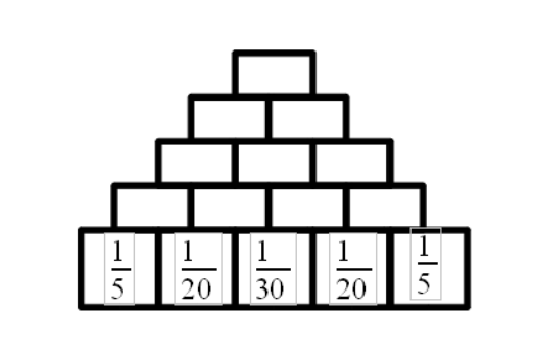
\includegraphics[scale=1.1]{pyramide.eps} 
\end{center}




\end{document}
